\section{Appendix}

\begin{lstlisting}[caption={`Greedy' Candidate Generation in DepDetector},captionpos=b,language=Python,label=lst:greedy-depdetector]
def get_greedy_candidates(root):
    convergence = True
    threshold = root.most_recent_nodes()[0].parent.score
    highscore_node = None

    for node in most_recent_nodes():
        if root.is_continuous:  # sequential RHS
            if (node.score <= 1.02*threshold) and (len(node.name) > 1):
                highscore_node = node
        elif not root.is_continuous:  # classifiable RHS
            if (node.score >= 0.98*highscore) and (len(node.name) > 1):
                highscore_node = node

    if highscore_node is not None:
        convergence = False
        pot_lhs = highscore_node.name
        for col in pot_lhs:
            candidate_lhs = [c for c in pot_lhs if c != col]
            add_node(candidate_lhs,
                     parent=highscore_node,
                     score=None)
\end{lstlisting}

\begin{figure}[ht]
     \centering
     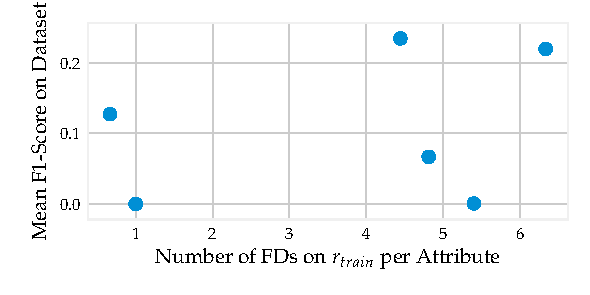
\includegraphics[width=.8\textwidth]{robustness-number-of-classifiable-fds.pdf}
     \caption{Mean robustness of all FDs with a classifiable RHS in function of the total number of FDs with a classifiable RHS divided by the total number of attributes in a dataset. No functional relation between these two values can be stated.}
     \label{fig:robustness-number-of-classifiable-fds}
 \end{figure}
